%copyright MJ Meintjes
%low level signal processing 
%included in skripsie.tex

\section{Overview}
The low-level signal processing module (LLSPM) extracts and amplifies
the EEG signal from the acquisition module output signal and reduces
the overall signal spectrum to the bandwidth of interest.

An instrumentation amplifier is deployed to isolate the differential
EEG signal from the common mode interference signal present at the
scalp surface. The cranial signal is applied to the instrumentation
amplifier inputs via the active electrodes described in
Chapter~\ref{chap:sa}. The resulting signal is band--limited by a set
of high and low--pass filters. Filtering the signal increases the
system signal to noise ratio by reducing the effective interference
bandwidth. The active and passive components in the filtering circuits
contributes to system noise levels lowering the SNR. Various
techniques and precautions are employed to reduce the filter and
differential stage system noise contributions.

DC components introduced by the instrumentation amplifier stage is
removed by applying a high-pass filter to the instrumentation
amplifier output. The high-pass filter output is amplified by a
variable amount before the signal is passed on to the next filter
stage.

A steep roll-off low-pass filter is employed to remove any signal
components above 50~Hz. A right-leg drive circuit is employed to
further minimize the common mode signal induced by power line and
fluorescent-light interference.


\section{LLSPM design specification}
The low-level signal processing module must be capable of extracting
and amplifying a 5~$\mu$V$_{pp}$ -- 100~$\mu$V$_{pp}$ signal from a
common mode signal several orders of magnitude larger. The resulting
differential signal must be amplified to within a -5~V~+~5~V range and
unwanted signal components removed. Care must be taken to reduce
signal noise and interference.

The LLSPM design specification is logically separated into a
differential signal extraction and a signal filtering submodule. The
design specification for each submodule is separately documented. The
convention of separately stating submodule specifications allows for
the substitution of any submodule with an alternative without adversely
affecting the overall system design. This keeps with the overall
modular tenet adhered to throughout the system design and
implementation process and may aid a process of comparative analysis
should such a requirement arise. The LLSPM must be housed in a small
EMI-resistant container and powered from the same battery pack as the
signal acquisition module.

\subsection{Differential amplifier design specification}
\label{section:dif-spec}
The differential amplifier stage of the LLSPM must reject common-mode
interference signals ($e_c$ Figure~\vref{fig:sme-eq}) and amplify the
differential EEG signal ($e_{EEG}$) as measured on the scalp
surface. In order to simplify design and increase signal quality a
commercial instrumentation amplifier device must be used. Because the
active electrodes employed in the signal acquisition module are AC
coupled (see Figure~\vref{fig:active-electrode}) the instrumentation
amplifier can be set close to its maximum gain setting without fear of
amplifier saturation or signal clipping. Setting gain close to maximum
enhances the CMRR and reduces the common mode interference
accordingly. The design must minimize the intrinsic system noise
contribution of the differential stage and component values must be
selected with cognizance of inherent component noise figures as noted
in Section~\vref{section:noise-analyses}. Table~\vref{table:df-specs}
summarizes the differential stage system parameters of the LLSPM
system specification.

\begin{table}
\begin{center}	
	\begin{tabular}[hpb]{|c|c|} \hline
	Parameter & Value \\ \hline
	Minimum CMRR & 100~dB \\
	Minimum Gain & 25~dB \\ 
	\hline
	\end{tabular}
	\caption{Differential amplifier specification}
	\label{table:df-specs}
\end{center}	
\end{table}



\subsection{Signal conditioning design specification}
\begin{figure}[htb]
\begin{center}
	\psfrag{G}[][]{$G$}
 	\psfrag{0db}[][]{0~dB} 
 	\psfrag{-3db}[][]{-3~dB} 
 	\psfrag{hpa}[][]{$A_{HPs}$} 
 	\psfrag{lpa}[][]{$A_{LPs}$} 
 	\psfrag{hps}[][]{$f_{HPs}$}
 	\psfrag{hpt}[][]{hp-trans} 
	\psfrag{fchp}[][]{$f_{HPc}$} 
	\psfrag{pb}[][]{Pass-band}
	\psfrag{f}[][]{f [Hz]}
	\psfrag{fclp}[][]{$f_{LPc}$}
	\psfrag{lpt}[][]{lp-trans}
	\psfrag{lps}[][]{$f_{LPs}$}
	\psfrag{rip}[][]{ripple}
	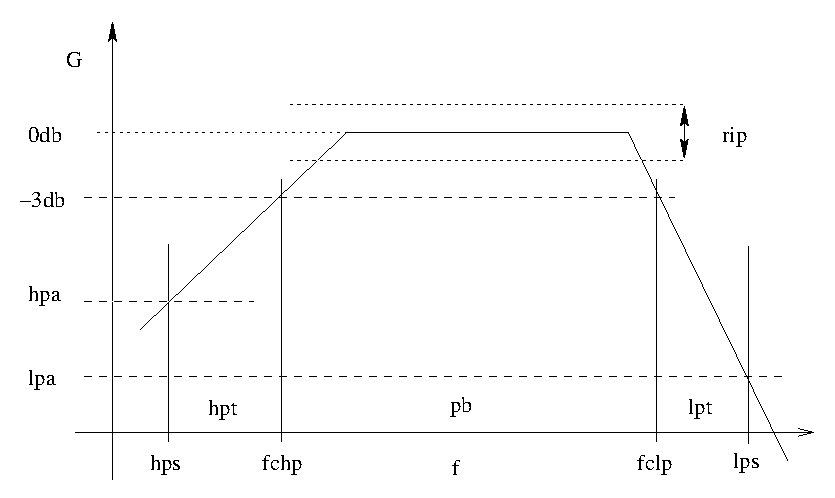
\includegraphics[width=\textwidth]{sig-cond-spec.eps}
	\caption{Signal conditioning specification}
	\label{fig:sig-cond-spec} 
\end{center}
\end{figure}

Figure~\vref{fig:sig-cond-spec} represents the frequency response
requirement for the signal conditioning submodule. The signal gain
($G$) is plotted against frequency from the high-pass filter stop
frequency $f_{HPs}$ to the low-pass filter stop frequency
$f_{LPs}$. The combination of the high-pass and low-pass filters acts
as a band-pass filter with the pass-band stretching from the high-pass
corner frequency $f_{HPc}$ to the low-pass corner frequency
$f_{LPc}$. The corner frequencies are chosen at the customary -3~dB or
half-power attenuation frequencies. Both filters have Butterworth
response characteristics as the $\pm$0.5~dB ripple budget is spent on
the active electrode response of Section~\ref{section:ae-imp}. The
amount of pass-band ripple contributed to the signal response must
therefore be 0~dB.

The slopes of the individual filters are determined by the attenuation
values $A_{HPs}$ and $A_{LPs}$ at the stop band frequencies $f_{HPs}$
and $f_{LPs}$. The slope specification determines the complexity of
the individual filters in number of pole
terms. Table~\vref{table:sc-specs} summarizes the chosen parameter
values indicated in Figure~\vref{fig:sig-cond-spec}.


\begin{table}
\begin{center}	
	\begin{tabular}[htpb]{|c|c|} \hline
	Parameter & Value \\ \hline
	$f_{HPs}$ & 0.05~Hz \\
	$f_{HPc}$ & 0.1~Hz \\ 
	$f_{LPc}$ & 35~Hz \\
	$f_{LPs}$ & 50~Hz \\
	$A_{HPs}$ & -40~dB \\
	$A_{LPs}$ & -50~dB \\
	\hline
	\end{tabular}
	\caption{Signal conditioning specification}
	\label{table:sc-specs}
\end{center}	
\end{table}

The high-pass corner frequency $f_{HPs}$ is chosen as 0.1~Hz in order
to include low $\delta$ frequency EEG signal information. Although
current EEG
research~\footnote{http://www.medizin.uni-tuebingen.de/medpsych/projekte/frequenc.htm}
suggests that human $\gamma$-band EEG activity is correlated with
abstract conceptualization, and does therefore contain relevant EEG
information, the low-pass filter is designed to attenuate all
frequencies above $f_{LPc}$. This decision simplifies system design
and implementation while retaining the bulk of EEG information used in
clinical practice for analysis and diagnosis.

The stop-band attenuation value for the low-pass filter $A_{LPs}$ is
dictated in part by the anti-aliasing requirements of the signal
conversion module of Chapter~\ref{chap:sc}. Because aliasing is a
fundamental mathematical result of the sampling process it is
preventable only by removing the frequency components above the
Nyquist frequency. For a signal undergoing A/D conversion the
amplitude of any frequency component above the Nyquist frequency
should at most influence only the least significant converter bit
\cite[p7]{design-guide}. Attenuation for frequencies above the Nyquist
frequency must be greater than 6$n$~dB with $n$ the bit resolution of
the converter. Because the EEG band is composed of low frequency
components (0.1~Hz~--~35~Hz) the sampling frequency can be set orders
of magnitude larger than $f_{LPc}$ negating most aliasing concerns.

The signal strength of the 50~Hz power line interference signal can be
significantly larger than that of the EEG signal
\cite{noise-rejection} \cite{fluorescent-interference}
\cite{fluorescent-interference2}, and must be effectively suppressed
to preserve signal quality and the system SNR.

\subsection{LLSPM container design specification}
In order to keep connecting signal wiring as short as possible both
the differential amplifier and signal conditioning submodules of the
LLSPM implementation must be situated physically near the SAM
container. To simplify construction and optimize space usage both
submodules will be contained in a single container. Grouping the
submodules together simplifies power and shielding requirements.


\section{LLSPM implementation}
\subsection{Differential Amplifier design and implementation}
\begin{figure}[htbp]
	\begin{center}
	\psfrag{vo}{$v_o$}
	\psfrag{r1}[][]{$R_1$} 
	\psfrag{r2}[][]{$R_2$} 
	\psfrag{r3}[][]{$R_3$} 
	\psfrag{r4}[][]{$R_4$} 
	\psfrag{r5}[][]{$R_5$} 
	\psfrag{r6}[][]{$R_6$} 
	\psfrag{r7}[][]{$R_7$} 
	\psfrag{c1}{$C_1$}
	\psfrag{c2}{$C_2$}
	\psfrag{+}{+}
	\psfrag{-}{--}
	\psfrag{1}{1}
	\psfrag{2}{2}
	\psfrag{3}{3}
	\psfrag{5}{5}
	\psfrag{8}{8}
	\psfrag{6}[][]{6}
	\psfrag{vae1}{$v_{AE_1}$}
	\psfrag{vae2}{$v_{AE_2}$}
	\psfrag{dr}{$drive$}
	\psfrag{AD620}{AD620}
	\psfrag{TL071}{071}
	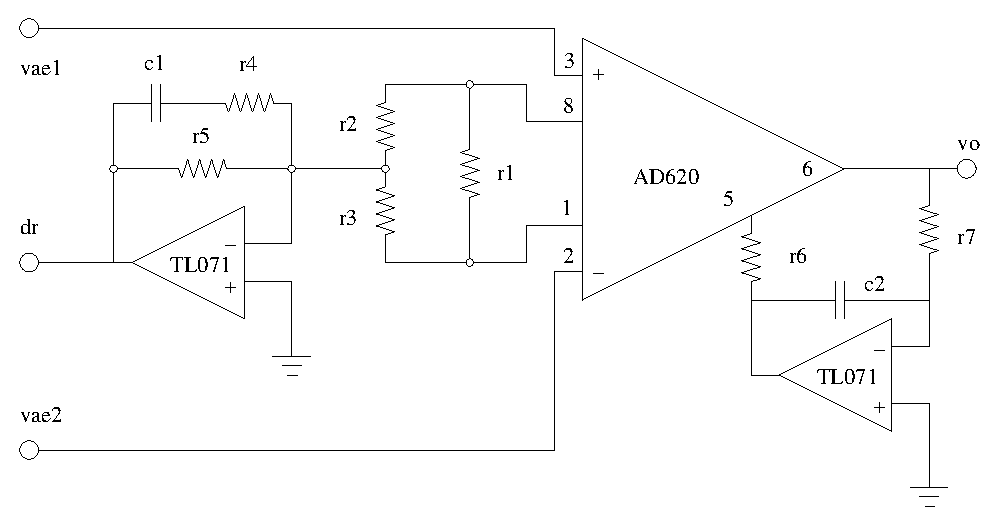
\includegraphics[width=\textwidth]{instrumentation-amp.eps}
	\caption{Differential amplifier implementation}
	\label{fig:instrumentation-amp} 
	\end{center}
\end{figure}

Figure~\vref{fig:instrumentation-amp} depicts the differential
amplifier sub-module deployed in the LLSPM. The differential stage is
implemented using the monolithic AD620 integrated instrumentation
amplifier available from Analog
Devices~\footnote{http://www.analog.com}. 

The AD620 consumes a maximum of 1.3~mA during normal operation making
it suitable for use in a battery operated system as specified in the
general LLSPM specification. The device has maximum nonlinearity of
40~parts per million, a maximum offset drift of
0.6~$\frac{\mu\/V}{^oC}$ and a maximum input offset value of
50~$\mu$V. The device has low input noise figures,
9~$\frac{nV}{\sqrt{Hz}}$ at 1~kHz, $\pm$0.28~$\mu\/V_{pp}$ in the
0.1~Hz~--~35~Hz band and 0.1~$\frac{pA}{\sqrt{Hz}}$ input current
noise~\footnote{AD620 data sheet}, which makes it suitable for use as
a pre-amplifier in the microvolt stages of a EEG signal amplitude
level (2~--~100~$\mu$V) data acquisition system.

The AD620 has a minimum CMRR of 110~dB ranging from DC to 60~Hz. This
performance specifications satisfies the differential amplifier design
specification noted in Section~\vref{section:dif-spec} and
Table~\ref{table:df-specs}.

\begin{table}
\begin{center}	
	\begin{tabular}[htpb]{|l|l|} \hline
	CMRR$_{min}$ (0 -- 60~Hz) & 110~dB \\
	Maximum Gain error ($\pm$10V) & 0.7\% \\
	$f_{-3~dB}$ & 12~kHz \\
	RTI (0.1~Hz -- 10~Hz) & 0.28~$\mu$V$_{p-p}$ \\
	\hline
	\end{tabular}
	\caption{AD620 specifications at $G = 500$}
	\label{table:ad620-1k}
\end{center}	
\end{table}
Table~\vref{table:ad620-1k} summarizes the relevant device
specifications as noted in the AD620 data sheet for a gain setting of
500.

The AD620's gain can be set accurately to within 0.15\% using a
single external gain resistor $R_g$. The gain resistance value is
calculated from the gain equation specified in the product data sheet:
\begin{equation}
	R_g = \frac{49.4~k\Omega}{G - 1}
	\label{eq:620-gain}
\end{equation}
With the device's gain set to $G = 500$, $R_g = 100~\Omega$. The gain
resistor $R_g$ is formed by the parallel $R_1$, $R_2$ and $R_3$
combination:
\begin{equation}
	R_g = \frac{R_1(R_1 + R_2)}{R_1 + R_2 + R_3}
	\label{eq:par}
\end{equation}
From Equation~\ref{eq:par} follows:
\begin{center}	
	\begin{tabular}[htpb]{|c|c|} \hline
	$R_1$ & 100~$\Omega$ \\
	$R_2$ & 100k~$\Omega$ \\
	$R_3$ & 100k~$\Omega$ \\
	\hline
	\end{tabular}
\end{center}	

The total resistance between pins 1 and 8 sets the AD620's gain value
to the value specified by Equation~\ref{eq:620-gain}. Where possible
1\% accurate metal film resistors where used.

\subsubsection{DC offset reduction}
The AD620 has a reference pin (5) from which can be used to set the
internal reference of the device. The output appearing at pin 6 is
referred to the voltage at pin 5. The DC--correcting circuit at the
AD620 output samples the output and feeds back a DC offset voltage to
the reference pin via the operational amplifier. This circuit
configuration reduces any DC offset voltages that may be present in
the output signal.

\begin{table}
\begin{center}	
	\begin{tabular}[htpb]{|l|l|} \hline
	$R_6$ & 10~k$\Omega$ \\
	$R_7$ & 1~M$\Omega$ \\
	$C_2$ & 300~nF \\
	\hline
	\end{tabular}
	\caption{AD620 reference pin driver}
	\label{table:dc}
\end{center}	
\end{table}

Table~\ref{table:dc} summarizes the component values of the reference
driver.

\subsubsection{Interference reduction}
The primary source of signal contamination in EEG acquisition systems
is environmental interference. The most prevalent sources of
interference are indoor power lines as well as fluorescent--light EMI
radiation. Power line interference is present as constant 50Hz signal
while the EMI radiated from the high--tension fluorescent--light coils
are present in the 1--10kHz range \cite{drive},
\cite{fluorescent-interference},
\cite{fluorescent-interference2}. These interference sources manifest
as large common mode voltage sources at the differential amplifier
inputs.

Due to non-linearities and component tolerances in the signal
acquisition paths the common mode voltage $v_c$ can be interpreted by
the instrumentation amplifier as a valid differential signal
\cite{drive}. 

In order to reduce $v_c$ a third electrode is used to provide a
low-impedance path between the subject and the amplifier
common. Directly connecting the electrode to the circuit ground is
undesirable for two reasons:
\begin{itemize}
	\item{A grounding electrode suffers from the same impedance
	problems as signal acquisition electrodes. A grounding electrode
	may represent up to 100k$\Omega$ between circuit ground and the
	subject's skin surface.}

	\item{Dangerous currents may flow through the grounding electrode
	if the patient should touch live power wiring. The threat of
	micro-shock is not as prevalent as in the case of ECG
	measurements, depending on the physical location of the grounding
	electrode, but may still lead to current burns.}
\end{itemize}

For these reasons the grounding electrode is usually driven by a
``right--leg drive circuit'' (RLD), named after the circuit's use in
ECG systems which uses a driven ground electrode attached to the
subjects right leg. The use of a driving circuit reduces the effective
electrode resistance by several orders of magnitude while allowing
only a save amount of current to flow through the grounding electrode.


\subsubsection{Right--leg drive design and implementation}

The reason for using a RLD circuit is to reduce $v_c$ to the lowest
possible level. Because of the exceptionally low voltage levels of EEG
signals (1--100~$\mu$V) a RLD needs to be optimally designed.

\subsubsection{Optimal Right--leg drive design}

The optimal RLD design was attempted according to a method by Winter
and Webster \cite{drive}.


\begin{figure}[htbp]
	\begin{center}
	\psfrag{i}[][]{100~nA}
	\psfrag{+}[][]{+}
	\psfrag{-}[][]{-}
	\psfrag{ad}[][]{$A_d$}
	\psfrag{ae}[][]{$A_e$}
	\psfrag{vo}[][]{$v_o$}
	\psfrag{vc}[][]{$v_c$}
	\psfrag{f}[][]{50~Hz}
	\psfrag{id}[][]{$i_d$}
	\psfrag{id1}[][]{$i_{d1}$}
	\psfrag{id2}[][]{$i_{d2}$}
	\psfrag{id3}[][]{$i_{d3}$}
	\psfrag{c1}[][]{$2~pF$}
	\psfrag{c2}[][]{$C_b$}
	\psfrag{re1}[][]{$R_{e1}$}
	\psfrag{ro}[][]{$R_o$}
	\psfrag{st}[][]{$S_1$}
	\psfrag{sg}[][]{$S_g$}
	\psfrag{rf}[][]{$R_f$}
	\psfrag{ra}[][]{$\frac{R_a}{2}$}
	\psfrag{c3}[][]{$2C_1$}
	\psfrag{c4}[][]{$C_s$}
	\psfrag{r1}[][]{$\frac{R_1}{2}$}
	\psfrag{re2}[][]{$\frac{R_{e2}}{2}$}
	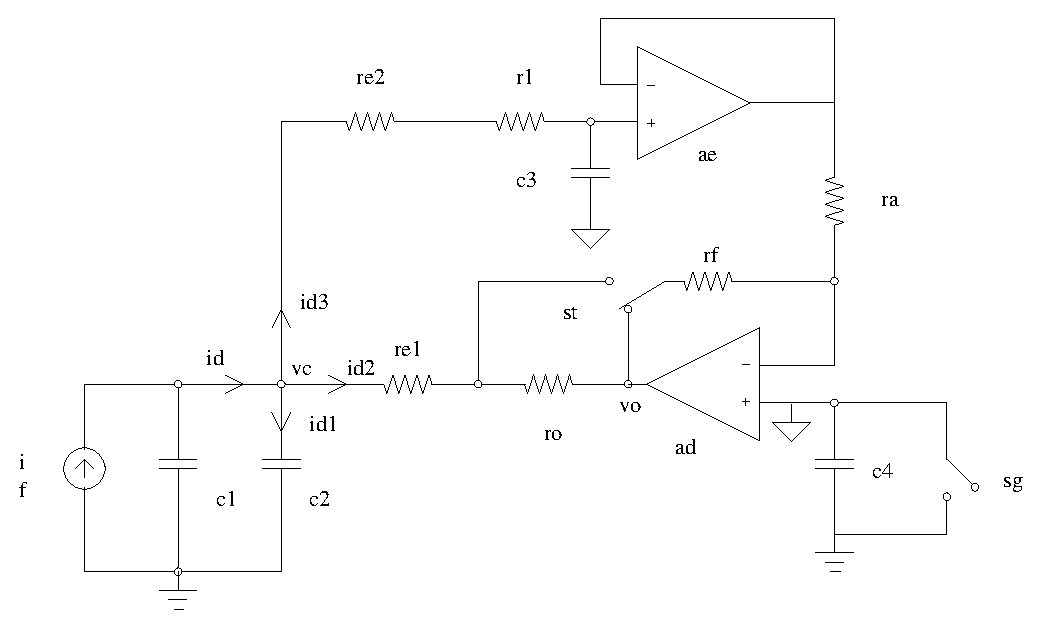
\includegraphics[width=\textwidth]{rld-opt1.eps}
	\caption{Right--leg drive equivalent circuit}
	\label{fig:rld-opt1} 
	\end{center}
\end{figure}


Figure~\vref{fig:rld-opt1} depicts the equivalent input side of the
differential input circuit of
Figure~\ref{fig:instrumentation-amp}. The averaging resistor
$\frac{R_a}{2}$ is equal to $\frac{R_2}{2}$ and $\frac{R_1}{2}$ of
Figure~\ref{fig:instrumentation-amp} ($R_1 = R_2 = 100~k\Omega$). The
electrode resistance $R_{e2}$ is the resistance introduced by the
stratum granulosum and is chosen as $100~k\Omega$. The low-pass filter
existing at the electrode input may be implemented in order to filter
out RF range frequencies. The RF interference could be demodulated by
the active electrodes into interference in the 0.1--35~Hz range. In
the implementation of the LLSPM these LP filters have been omitted as
they impair the effective CMRR of the amplifier at higher frequencies.

A low--pass filter due to parasitic capacitances between the cable
lead and common already exist at the input side of the operational
amplifier. The $R_1$ and $C_1$ values are lumped equivalents of a
implemented as well as the ever--present parasitic lead filter.

With the switch $S_g$ open the circuit of Figure~\ref{fig:rld-opt1}
represents an isolated amplifier with $C_s$ a stray capacitance to
environment ground. The capacitance between environment ground and the
subject is represented by $C_b$.

The object of a optimal RLD design is to calculate values for $R_o$
and $R_f$ for which the common mode voltage $v_c$ will be a minimum.


A displacement current $i_d$ flows between nearby power lines and the
body of the subject via stray capacitances. The capacitances are
lumped together as a 2~pF capacitor and exists in parallel with a
100~nA 50~Hz current source. The current $i_{d3}$ flowing into the
active electrode is assumed to be at least a order of magnitude
smaller that the $i_{d2}$ current flowing via the RLD to ground, that
is $i_{d3}~<<~i_{d2}$. The displacement current divides into $i_{d1}$
which flows directly to ground via $C_b$ and the $i_{d2}$ current
which flows to ground via the RLD circuit as follows:
\begin{equation}
	i_{d2} = \frac{i_dC_s}{C_s + C_b}
	\label{eq:id2}
\end{equation}

The gain ($G$) of the RLD amplifier $A_d$ is determined by $R_a$ and
$R_f$ with the normal inverting amplifier equation:
\begin{equation}
	G = \frac{2R_f}{R_a}
	\label{eq:G}
\end{equation}

From Equation~\ref{eq:G} follows the output voltage of $A_d$ ($v_o$):
\begin{equation}
	v_o = -Gv_c = v_c - (R_o + R_{e1})i_{d2}
	\label{eq:vo}
\end{equation}
With $R_{e1}$ the ground electrode resistance and $R_o$ the output
current limiting resistor.

From Equation~\ref{eq:G} and Equation~\ref{eq:vo} follows a expression
for $R_c$ the equivalent common mode resistance:
\begin{equation}
	R_c = \frac{R_o + R_{e1}}{G + 1}
	\label{eq:rc}
\end{equation}
From which follows that $v_c = R_ci_{d2}$.

If the ground electrode is directly connected to circuit ground
(common) the effective resistance between the subject and common is
$R_{e1}$, the electrode resistance. If the ground electrode is driven
by a RLD circuit like that of Figure~\ref{fig:rld-opt1} and $G >
\frac{R_o}{R_{e1}}$, the effective resistance is $R_c$, reducing the
common mode voltage $v_c$. The common mode voltage may also be reduced
by decreasing the isolation capacitance $C_s$ with respect to the body
capacitance $C_b$.


Good amplifier isolation is essential for subject or patient
safety. International respected standards
(NFPA)\footnote{http://www.nfpa.org/About\_NFPA/about\_nfpa.html}
require that less than 20~$\mu$A of current flow through any connecting
leads should the patient come in contact with power line voltage. This
includes the two sensing electrodes as well as the ground electrode.

If switch $S_g$ is closed somehow (common = environmental ground) the
design must ensure that at least 11~M$\Omega = (\frac{220V}{20\mu\/A})$
of impedance exists between all amplifier leads and ground. The output
resistance $R_o$ can be increased to limit current flowing through the
RLD circuit, it does however not ensure save current levels through
the sensing electrodes.

The isolation capacitance must be low enough to ensure that only the
allowed current flows should a power line voltage appear on the
amplifier: $C_s < \frac{20~\mu\/A}{(2\pi\/50)(220~V)} =
260~pF$\footnote{South--African conditions}. This means that isolated
amplifiers with $C_s < 260~pF$ do not require $R_o$ to reduce current
flow from external sources. The necessity of using $R_o$ to protect
against transient currents during startup or shutdown is doubtful as
current flow of up to 5~mA for a duration of less than 200~ms does not
seem to pose a micro-shock hazard \cite{drive}.

Should $R_o$ be included, the RLD circuit can be improved by switching
$S_1$ to the up position. The circuit will now measure the voltage at
the electrode in stead of $A_d$'s output. The ground electrode voltage
is now $-Gv_c$ and $R_c$ is independent of $R_o$: $R_c =
\frac{R_{e1}}{G + 1}$. For large gain ($G$) values $v_c$ is inversely
proportional to the gain. That is to minimize $v_c$ the gain must be
maximized.

The RLD maximum gain value is limited by the circuit's stability. For
the RLD to oscillate a $-180^o$ phase shift must be introduced
somewhere in the circuit. As the active electrodes have unity gain
they do not contribute much phase shift in the 0.1--35~Hz band of
interest. The RLD's $A_d$ amplifier does however introduce a pole at
$f = \frac{B}{G}$ with $B$ the gain-bandwidth product of $A_d$,
(3~MHz)\footnote{TL071 data-sheet} and $G = \frac{2R_f}{R_a}$.



\begin{figure}[htbp]
\begin{center}
	\psfrag{+}[][]{+}
	\psfrag{-}[][]{-}  
	\psfrag{s2}[][]{$S_2$} 
	\psfrag{vc1}[][]{$v_{c1}$}
	\psfrag{vc2}[][]{$v_{c2}$}  
	\psfrag{ad}[][]{$A_d$} 
	\psfrag{r1}[][]{$R_o + R_{e1}$}
	\psfrag{r2}[][]{$\frac{R_{e2} + R_1}{2}$}
	\psfrag{c1}[][]{$\frac{C_bC_s}{C_b + C_s}$}
	\psfrag{c2}[][]{$2C_1$}    
	\psfrag{ae1, ae2}[][]{$A_{e1}, A_{e2}$} 
	\psfrag{g1}{$\frac{G}{1 + \frac{G}{2\pi\/B}s}$}
	\psfrag{g2}{$\frac{G}{1 + \frac{1}{2\pi\/B}s}$}
	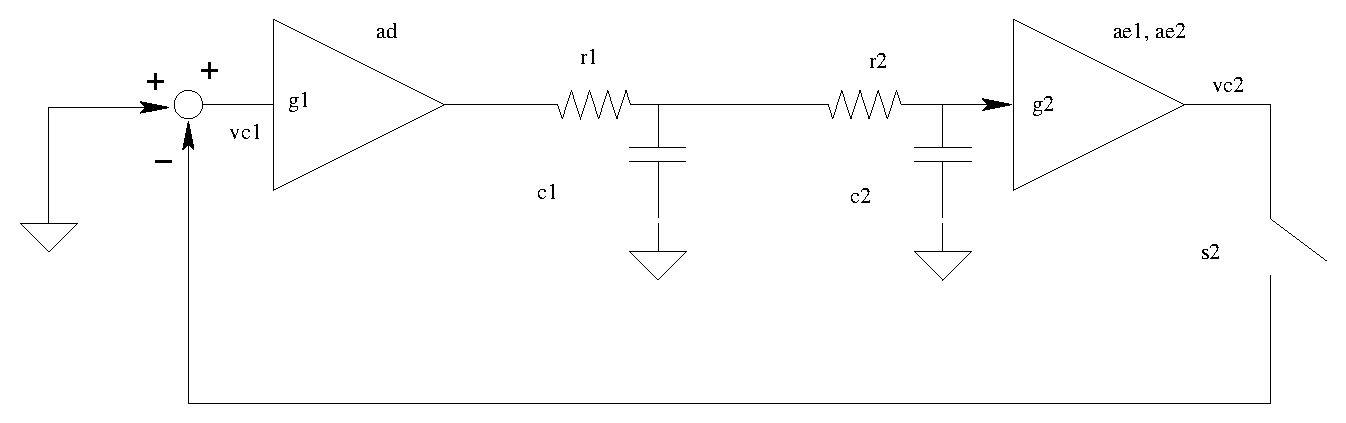
\includegraphics[width=\textwidth]{rld-gain.eps}
	\caption{Right-leg drive equivalent gain loop}
	\label{fig:rld-gain} 
\end{center}
\end{figure}

From Figure~\ref{fig:rld-gain} can be seen that two RC stages exist
which may introduce additional phase shifts in the RLD gain loop. The
first stage consist of the $R_o + R_{e1}$ series combination forming a
low pass filter with the $C_b + C_s$ combination. The other stage
consists of the $R_1 - C_1$ low pass filter discussed previously.

The low--frequency open--loop gain for the circuit depicted in
Figure~\ref{fig:rld-gain} is:


\begin{equation}
	\frac{v_{c1}}{v_{c2}} = \frac{G}{(1 + \frac{s}{2\pi\/f_a})(1 +
	\frac{ks}{2\pi\/f_n})(1 + \frac{s}{2\pi\/kf_n})}
	\label{eq:rld-gain}
\end{equation}

With $f_a$ the corner frequency of $A_d$ ($\frac{B}{G}$) and $B$ the
gain -- bandwidth product of $A_d$, and:
\begin{equation}
	G = \frac{2R_f}{R_a}
\end{equation}

\begin{equation}
	f_n = \frac{1}{2\pi\sqrt{\tau_1\tau_2}}
\end{equation}

\begin{equation}
	k = \zeta + \sqrt{\zeta^2 - 1}
\end{equation}

\begin{equation}
	\zeta = (\tau_1 + \tau_2 + \tau_3)\pi\/f_n
\end{equation}


The time constant for the first RC stage in Figure~\ref{fig:rld-gain}:
\begin{equation}
	\tau_1 = (R_o + R_{e1})\frac{C_bC_s}{C_b + C_s}
\end{equation}

The time constant for the second RC stage in Figure~\ref{fig:rld-gain}:
\begin{equation}
	\tau_2 = (R_{e2} + R_1)C_1
\end{equation}

The time constant $\tau_3$ relates how the second stage impedance loads
the first stage impedance:
\begin{equation}
	\tau_3 = 2(R_o + R_{e1})C_1
\end{equation}

If the loading effects of the second RC stage on the first RC stage
can be ignored, that is $\tau_3 << \tau_1$ or $\tau_3 << \tau_2$ then
Equation~\ref{eq:rld-gain} can be reduced to:
\begin{equation}
	\frac{v_{c2}}{v_{c1}} = \frac{G}{(1 + \frac{s}{2\pi\/f_a})(1 +
	s\tau_1)(1 + s\tau_2)}
\end{equation}

In order to keep the gain as high as possible while avoiding
oscillation the RLD is stabilized by using lag compensation. Lead
compensation is more difficult as the RLD circuit poles depend on
$R_{e1}$, $R_{e2}$ and $C_b$, which are variable depending on
environmental conditions.


In order to introduce lag compensation the corner frequency of the RLD
is lowered from $f_a$ to $f_{ac}$. The feedback impedance $R_f$ is can
be replaced with a capacitor $C_f$ as DC gain need not be limited.

The feedback capacitance in the RLD for the circuit in
Figure~\ref{fig:instrumentation-amp} is calculated using the following
values:
\begin{table}
\begin{center}	
	\begin{tabular}[htpb]{|c|c|} \hline
	$C_s$ & 200~pF \\
	$R_{e1}$, $R_{e2}$ & $1~\Omega$ \\
	$C_b$ & 200~pF \\
	$R_o$ & 10~k \\
	$C_1$ & 200~pF \\
	$R_1$ & 10~k \\
	\hline
	\end{tabular}
	\caption{RLD $C_f$ design values}
	\label{table:rld-cf}
\end{center}	
\end{table}

The values are chosen for a worse case scenario. From the above
follows that:

\begin{table}
\begin{center}	
	\begin{tabular}[htpb]{|c|c|} \hline
	$\tau_1$ & $1.001~\mu\/s$ \\
	$\tau_2$ & $2.002~\mu\/s$ \\
	$\tau_3$ & $4.004~\mu\/s$ \\
	$k$ & 4.7387 \\
	$f_n$ & 11.234~kHz \\
	\hline
	\end{tabular}
	\caption{RLD design constants}
	\label{table:rld-cfc}
\end{center}	
\end{table}

Seeing that the RC poles differ by more than a decade $f_ac$ must be
chosen in such a manner that the open loop gain of the RLD circuit has
at least a $45^o$ phase margin. With $f_{ac}$ the corner frequency of
$A_d$ with $C_f$ the capacitor in the feedback path:
\begin{equation}
	f_{ac} = \frac{1}{\pi\/G_oR_aC_f}
\end{equation}

With $f_L$ the lowest RC pole, that is:
\begin{equation}
	f_L = \frac{f_n}{k}
\end{equation}
And $G_o$ the low--frequency open loop gain of $A_d$:
\begin{equation}
	R_aC_f > \frac{k}{\pi\/f_n} = 134,2~\mu\/s
	\label{eq:rld-cf}
\end{equation}

\subsubsection{RLD bandwidth}
The gain of the RLD circuit at frequencies other than 50~Hz will
influence the reduction of interference at those frequencies. A large
contributer of high--frequency interference is fluorescent light
sources. Fluorescent light sources emit interference in the 1--10~kHz
range at a 100~Hz rate (2$f_l$, where $f_l$ is the power line
frequency, 50~Hz in South Africa). Parasitic low--pass filters at the
AD620 input may lower the CMRR for higher frequencies. For this reason
low pass filters were omitted from the IA front--end although they are
present in many commercial EEG systems. In order to reduce the
influence of high--frequency interference the bandwidth of the RLD must
include these interference frequencies.


\subsubsection{RLD realization}

\begin{figure}[htbp]
\begin{center}
	\psfrag{dr}[][]{$drive$}
	\psfrag{vc}[][]{$mv_c$}  
	\psfrag{r5}[][]{$R_5$} 
	\psfrag{r4}[][]{$R_4$} 
	\psfrag{ro}[][]{$R_o$} 
	\psfrag{c1}{$C_f$}
	\psfrag{+}{+}
	\psfrag{-}{--}
	\psfrag{TL071}{071}
	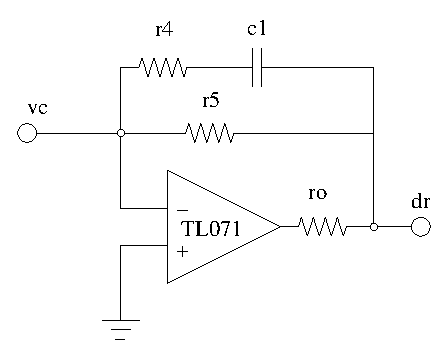
\includegraphics{rl-drive.eps}
	\caption{RLD drive circuit}
	\label{fig:rl-drive} 
\end{center}
\end{figure}


Figure~\vref{fig:rl-drive} represents the right-leg drive circuit of
Figure~\ref{fig:instrumentation-amp}. The circuit is realized using a
low-noise TL071 operational amplifier deployed as a inverting
integrating amplifier. The right-leg drive (RLD) circuit measures the
average of the common mode signal from the voltage tap created by the
$R_2$~--~$R_3$ voltage divider of
Figure~\vref{fig:instrumentation-amp}. The measured voltage is
inverted, amplified and fed back to the skin surface via the $drive$
electrode.

Non-optimal $v_c$ reducing RLD circuits seem to function as well or
within component error margins as that of optimally designed circuits
when used in ECG recording circuits \cite{drive}. However, for the
sensitive recording requirements of a EEG a optimally designed
right-leg drive is required to obtain the full noise suppression
capability potentially available from a optimally designed RLD. A
optimal circuit has the maximum gain allowed by the equations
governing the circuit's stability. 

The circuit bandwidth must allow for the inclusion and reduction of
fluorescent light interference frequencies. Circuit stability depends
on electrode resistance, RF interference and circuit decoupling
capacitance. The active electrodes described in Chapter~\ref{chap:sa}
reduces electrode resistance to less than 1~$\Omega$ and contributes
significantly to the stability of the RLD circuit \cite{drive}.


Component values were chosen as suggested by Equation~\ref{eq:rld-cf}
as well as the AD620 data sheet, $C_1$ is chosen to maintain stability
of the feedback loop.

\begin{table}
\begin{center}	
	\begin{tabular}[htpb]{|c|c|} \hline
	$R_4$ & 10~k$\Omega$ \\
	$R_5$ & 1~M$\Omega$ \\
	$C_f$ & 1~$\mu$F \\
	$R_o$ & $5~M\Omega$\\
	\hline
	\end{tabular}
	\caption{Right-leg drive component values}
	\label{table:rld}
\end{center}	
\end{table}

Table~\vref{table:rld} summarizes the component values used in the
right-leg drive circuit implementation.




\subsection{Signal Conditioning}
The differential amplifier output signal consists of the EEG
information in the band of interest (0.1~Hz~-~35~Hz), as well as
interference components above 35~Hz and DC components below
0.1~Hz. The undesirable signal components are removed by filtering the
differential signal through a set of active filters. Filtering
confines the signal bandwidth to the band of interest and enhances the
signal to noise ratio by reducing out of band noise. The resulting
signal is amplified and buffered to protect against possible loading
effects from subsequent system modules.

The active filters used in the LLSPM is implemented using standard
Sallen-Key filter architecture. This design is chosen for its
simplicity and low parts count \cite[p273]{art}. Care is taken to
compensate for the architecture's sensitivity to component variations
by using high-accuracy components where possible.


\subsection{Sallen-Key filter analysis}
\label{section:sk}
\begin{figure}[htbp]
	\psfrag{vi}{$v_i$}
	\psfrag{vo}{$v_o$}
	\psfrag{ve}{$v_e$}
	\psfrag{z1}{$Z_1$}
	\psfrag{z2}{$Z_2$}
	\psfrag{z3}{$Z_3$}
	\psfrag{z4}{$Z_4$}
	\psfrag{a}{$a$}
	\psfrag{b}{$b$}
	\psfrag{c}{$c$}
	\psfrag{r4}{$R_4$}
	\psfrag{r3}{$R_3$}
	\psfrag{+}{+}
	\psfrag{-}{--}
	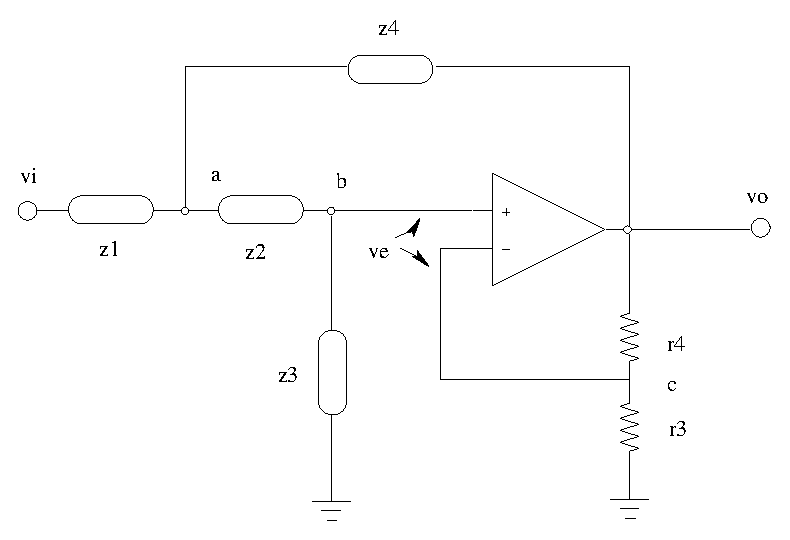
\includegraphics{sallen-key-gen.eps}
	\caption{Sallen-Key architecture.}
	\label{fig:sallen-key} 
\end{figure}

The operation of Sallen-Key filters are based on positive feedback
localized to the filter corner frequency $f_c$
\cite[p1]{sk-analysis}. Positive feedback enables the filter $Q$ to
be extended well above that of passive filters \cite[p267]{art}.

Figure~\vref{fig:sallen-key} depicts the general form of the
Sallen-Key architecture. $R_3$ and $R_4$ creates a non-inverting
voltage amplifier with frequency independent gain $K$. $Z_1$ to $Z_4$
dictates the frequency response characteristics of the filter. The
general 2-pole form of Figure~\vref{fig:sallen-key} is cascaded in
series to form more complex multi-pole filters with any of the
standard Butterworth, Chebyshev or Bessel responses. Each 2-pole
filter stage in a multi-pole filter represents a quadratic polynomial
factor of the $n$'th order polynomial describing the overall filter
transfer function \cite[p274]{art}.

\subsubsection{ Sallen-Key transfer function}
Determining the relationship between $v_i$, $v_o$, $v_b$ and $v_a$
allows the construction of a system gain-block diagram. Describing the
the system in this manner enables the formulation of a general
transfer function easily adopted to different filter configurations.

\begin{figure}[htbp]
	\psfrag{vo}{$v_o$}
	\psfrag{vi}{$v_i$}
	\psfrag{ve}{$v_e$}
	\psfrag{af}{$p(f)$}
	\psfrag{d}{$q$}
	\psfrag{b}{$r$}
	\psfrag{c}{$s$}
	\psfrag{+}[][]{+}
	\psfrag{-}[][]{--}
	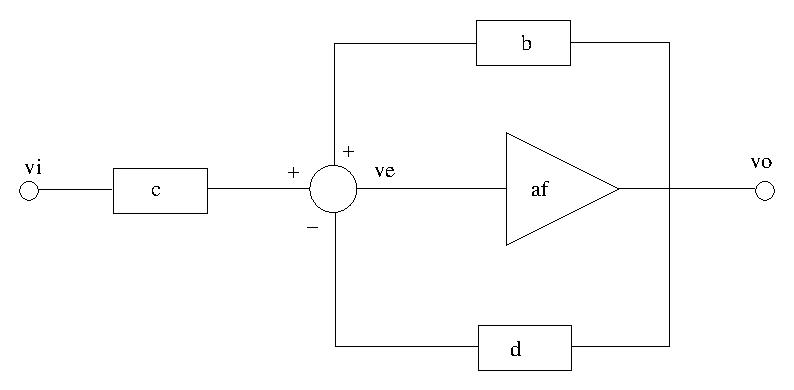
\includegraphics{sk-block.eps}
	\caption{Sallen-Key gain-block diagram.}
	\label{fig:sk-block} 
\end{figure}

Figure~\vref{fig:sk-block} represents the equivalent gain-block
diagram of the Sallen-Key filter described in
Figure~\vref{fig:sallen-key}. The gain values ($p$, $q$, $r$, $s$) in
Figure~\ref{fig:sallen-key} are determined by summing currents at
nodes $a$, $b$ and $c$ in Figure~\vref{fig:sk-block}. The relationship
between the node voltages are described in terms of the calculated
gain values in the feedback and forward-feed paths of the gain-block
diagram:
\begin{equation}
	v_e = sv_i + rv_o - qv_o	
	\label{eq:sk-t1}
\end{equation}
\begin{equation}
	v_o = p(f)v_i
	\label{eq:sk-t2}
\end{equation}
With $p(f)$ the open loop gain of the operational amplifier ($p(f) =
A_{open-loop}$). The frequency independent feedback gain $q$ through
$R_3$ and $R_4$ is that of the standard non-inverting operational
amplifier gain.
\begin{equation}
	q = \frac{R_3}{R_3 + R_4}
\end{equation}
The forward-feed gain of the input signal $v_i$ in terms of the $Z$
impedances.
\begin{equation}
	s = \frac{Z_2Z_3Z_4}{Z_2Z_3Z_4 + Z_1Z_2Z_4 + Z_2Z_3Z_1 + Z_2Z_2Z_4
	+ Z_2Z_2Z1}
\end{equation}
The feedback gain of the output signal $v_o$ in terms of the $Z$
impedances.
\begin{equation}
	s = \frac{Z_1Z_2Z_3}{Z_2Z_3Z_4 + Z_1Z_2Z_4 + Z_2Z_3Z_1 + Z_2Z_2Z_4
	+ Z_2Z_2Z1}
\end{equation}
Describing the circuit of Figure~\vref{fig:sallen-key} in voltage gain
terms simplifies the adaption of the general circuit transfer function
to either low or high-pass behavior. From Figure~\ref{fig:sallen-key}
and Equations~\ref{eq:sk-t1} and \ref{eq:sk-t2} the general Sallen-Key
filter transfer function is described as follows:
\begin{equation}
	\frac{v_o}{v_i} = \frac{s}{q}\left( \frac{1}{1 + \frac{1}{p(f)q}
	-\frac{r}{q}}\right ) 
	\label{eq:sk-trans}
\end{equation}
For a idealized operational amplifier the open loop gain
$p(f)~\rightarrow~\infty$ or
$\frac{1}{p(f)}~\rightarrow~0$. Substituting the impedance terms into
the idealized Equation~\ref{eq:sk-trans} leads to the general
Sallen-Key filter transfer function:
\begin{equation}
\frac{v_o}{v_i} = \frac{K}{\frac{Z_1Z_2}{Z_3Z_4} + \frac{Z_1}{Z_3} +
\frac{Z_1(1 - K)}{Z_4} + 1}
	\label{eq:sk-gen-tans}
\end{equation}
With $K = \frac{1}{q} = \frac{R_3}{R_3 + R_4}$, the frequency
independent feedback gain.

\subsection{High--pass filter design and implementation}
The resulting differential signal from the instrumentation amplifier
output may have a small DC offset voltage due to gain differences and
bias currents in the differential input buffer stages. The offset
voltage is normally very low due to the monolithic nature of the
instrumentation amplifier.

\begin{figure}[htbp]
	\psfrag{vo}{$v_o$}
	\psfrag{vi}{$v_i$}
	\psfrag{r1}[][]{$R_1$} 
	\psfrag{r2}[][]{$R_2$} 
	\psfrag{r3}[][]{$R_3$} 
	\psfrag{r4}[][]{$R_4$} 
	\psfrag{c2}[][]{$C_2$} 
	\psfrag{c1}{$C_1$}
	\psfrag{+}{+}
	\psfrag{-}{--}
	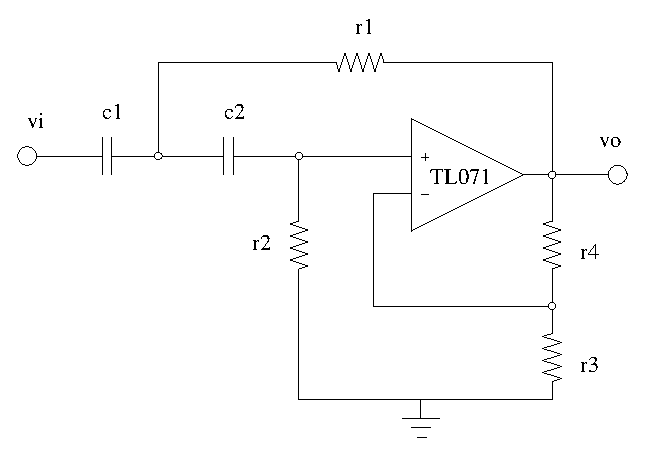
\includegraphics{high-pass.eps}
	\caption{Sallen-Key two-pole high-pass filter}
	\label{fig:high-pass} 
\end{figure}

The high pass-filter is implemented using the Sallen-Key architecture
described in Section~\vref{section:sk} with the $Z$ impedances adopted
for a high-pass filter response. Figure~\vref{fig:high-pass}
represents the circuit diagram for a Sallen-Key high-pass filter.

With $K = 1 + \frac{R_4}{R_3}$, $Z_3 = R_2$, $Z_4 = R_1$, $Z_2 =
\frac{1}{sC_2}$ and $Z_1 = \frac{1}{sC_1}$ the general transfer
function of Equation~\ref{eq:sk-trans} becomes:
\begin{equation}
	H(s)_{hp} = \frac{K(s^2R_1R_2C_1C_2)}{s^2(R_1R_2C_1C_2) + s(R_2C_2
	+ R_2C_1 + R_1C_2(1 - K) + 1)}
	\label{eq:lp-t1}
\end{equation}
Equation~\ref{eq:lp-t1} is significantly simplified by setting the
filter components as equal, $R_1 = R_2 = R$ and $C_1 = C_2 =
C$. Equating component values in this manner reduces system component
diversity and simplifies filter construction.
\begin{equation}
	H(s)_{hp} = \frac{Ks^2(RC)^2}{(RC)^2s^2 + s(2RC + RC(1 - K) + 1)}
	\label{eq:simp-hp}
\end{equation}
The filter design equations are reduced to simple relationships
describing the filter's $Q$ and corner frequency $f_c$.
\begin{equation}
	f_c = \frac{1}{2\pi\/RC}
	\label{eq:hp-fc}
\end{equation}

\begin{equation}
	Q = \frac{1}{3 - K}
	\label{eq:hp-q}
\end{equation}

Equation~\ref{eq:hp-q} illustrates the circuit's $Q$ dependence on the
gain value $K$ only, a additional gain stage must be used to achieve
the desired signal amplification. Because $f_c$ and $Q$ are
independent the filter transfer function can be manipulated to
represent any of the standard filter types. The high-pass filter
functions as expected in the low frequency (0.1~Hz--35~Hz) EEG
bandwidth. The filter has a upper cutoff frequency determined by the
open loop response of the operational amplifier. The TL071 device has
a low--pass cutoff of approximately 100~kHz.

The filter's departure from the ideal transfer function described in
Equation~\ref{eq:simp-hp} does not influence the EEG signal within the
bandwidth of interest.

\subsubsection{High-pass filter implementation}
A single two-pole filter stage is used in the high-pass filter
implementation. In order to preserve the flatness of the response
obtained from the active electrode described in Chapter~\vref{chap:sa}
a Butterworth response is chosen.

From \cite[p274]{art} Table~5.2 the gain $K$ is chosen as 1.586,
applying Equation~\ref{eq:hp-q} results in a $Q$ factor of
0.707. Choosing $C_1 = C_2$~=~2$\mu$F and applying
Equation~\ref{eq:hp-fc} results in $R_1 = R_2$~=~800~k$\Omega$. For
$R_4$~=~10~k$\Omega$, $R_3$ results in 17~k$\Omega$.


\begin{table}
\begin{center}	
	\begin{tabular}[htpb]{|c|c|c|c|} \hline
	Component & Value \\ \hline
	$C_1 = C_2$ & 2~$\mu$F \\
	$R_1 = R_2$ & 800~k$\Omega$ \\ 
	$R_4$ & 10~k$\Omega$ \\
	$R_3$ & 17~k$\Omega$ \\
	\hline
	\end{tabular}
	\caption{High-pass filter component values}
	\label{table:hp-comp}
\end{center}	
\end{table}
Table~\vref{table:hp-comp} is a summary of the component values used in
the high-pass filter implementation. Polyethylene capacitors and 1\%
accurate metal film resistors are used.


\subsection{Low--pass filter design and implementation}
\begin{figure}[htbp]
	\psfrag{vi}[][]{$v_i$} 
	\psfrag{vo}[][]{$v_o$}
	\psfrag{r1}[][]{$R_1$} 
	\psfrag{r2}[][]{$R_2$}
	\psfrag{r3}[][]{$R_3$} 
	\psfrag{r4}[][]{$R_4$} 
	\psfrag{c1}[][]{$C_1$}
	\psfrag{c2}[][]{$C_2$} 
	\psfrag{+}[][]{+} 
	\psfrag{-}[][]{--} 
	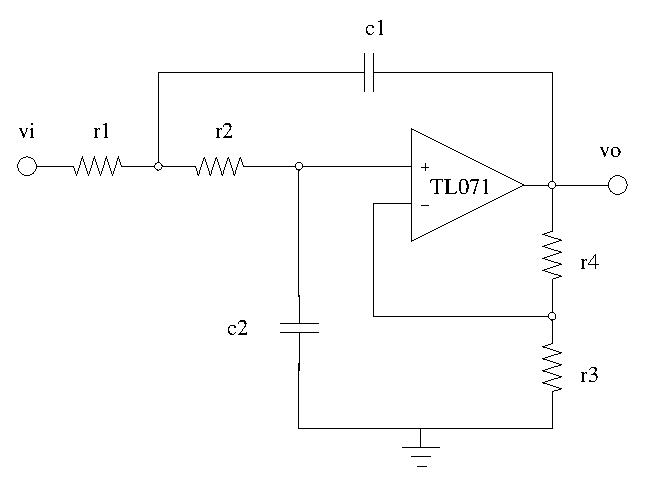
\includegraphics{low-pass.eps} 
	\caption{Sallen-Key two-pole low-pass filter.}  
	\label{fig:low-pass}
\end{figure}

The low-pass filter used in the signal conditioning sub-module is
required to reduce all signal components at 50~Hz to a minimum of
-72~dB. The strongest interference component attributed to power line
induction is encountered at 50~Hz and harmonics thereof. The roll-off
of the filter response from pass-band (35~Hz) to stop-band (50~Hz) is
steep and requires a fairly complex filter.

The low-pass filter is implemented using the Sallen-Key architecture
described in Section~\vref{section:sk} with the $Z$ impedances adapted
for a low-pass filter response. Figure~\vref{fig:low-pass} represents
the circuit diagram for a two-pole Sallen-Key low-pass filter.

With $K = 1 + \frac{R_4}{R_3}$, $Z_1 = R_1$, $Z_2 = R_2$, $Z_3 =
\frac{1}{sC_1}$ and $Z_4 = \frac{1}{sC_2}$ the general transfer
function of Equation~\ref{eq:sk-trans} becomes:
\begin{equation}
	H(s)_lp = \frac{K}{s^2(R_1R_2C_1C_2) + s(R_1C_2 + R_2C_2 +
	R_1C_1(1 - K) + 1)}
	\label{eq:hs-lp}
\end{equation}
Equation~\ref{eq:hs-lp} is significantly simplified by equating the
filter passive component values. By letting $C_1 = C_2 = C$ and $R_1 =
R_2 = R$ the filter's component diversity is reduced and the
implementation significantly simplified.
\begin{equation}
	H(s)_lp = \frac{1}{(RC)^2s^2 + s(2RC + RC(1 - K) + 1)}
	\label{eq:hs-lp2}
\end{equation}
The filter design equations are once more reduced to simple
relationships describing the filter's $Q$ and corner frequency
$f_c$. These relationships are identical to those describing the
high-pass filter's gain $K$ and quality factor $Q$ relationship, as
well ass the corner frequency $f_c$.
\begin{equation}
	f_c = \frac{1}{2\pi\/RC}
	\label{eq:lp-fc}
\end{equation}

\begin{equation}
	Q = \frac{1}{3 - K}
	\label{eq:lp-q}
\end{equation}

$f_c$ and $Q$ are independent the filter transfer function can be
manipulated to represent any of the standard filter types. The
low-pass filter functions as expected in the low frequency
(0.1~Hz--35~Hz) EEG bandwidth. For very high frequencies into the stop
band the filter acts as a high-pass filter due to non-linearities in
the open-loop output impedance. This departure from the ideal transfer
function does not influence the filter action in the band of interest.

\subsubsection{Low-pass filter implementation}
Multiple two-pole stage low-pass filters are cascaded in series to
obtain the necessary roll-off from the pass-band to the stop-band as
prescribed in the LLSPM specification in
Figure~\vref{fig:sig-cond-spec}. The filter is designed with a
Butterworth response in order to preserve the flatness of the total
system response. Choosing the a Butterworth response for the low-pass
filter in order to preserve flatness increases system complexity in
terms of component usage as well as system noise.

For the specified low-pass filter corner frequency $f_c = 35$~Hz and a
chosen capacitor value $C_1 = C_2 = 2\mu$~F, Equation~\ref{eq:lp-fc}
results in $R_1 = R_2 = 2.273$~k$\Omega$. From Table~5.2
\cite[p274]{art} the gain values $K$ for a ten-pole Butterworth filter
is chosen as specified per pole-pair. A two-pole set in series with a
eight-pole set is chosen and implemented as a single two-pole low-pass
Butterworth filter. The gain values are chosen for maximal gain in the
early stages in order to minimize noise amplification in the latter
filter stages.

The frequency-independent feedback loop formed by $R_4$ and $R_3$ gain
resistors are specified by the $R_4 = (K - 1)R_3$ relationship. The
filter is implemented using the low noise ($V_n =
18~\frac{nV}{\sqrt{Hz}}$) TL071 operational amplifier from Texas
Instruments, low-noise 1\% metal film resistors and low-drift
polypropylene capacitors.

\begin{figure}[htbp]
	\psfrag{TL071}[][]{071} 
	\psfrag{1}[][]{1} 
	\psfrag{2}[][]{2} 
	\psfrag{3}[][]{3} 
	\psfrag{4}[][]{4} 
	\psfrag{5}[][]{5} 
	\psfrag{vi}[][]{$v_i$} 
	\psfrag{vo}[][]{$v_o$}
	\psfrag{r1}[][]{$R_1$} 
	\psfrag{r2}[][]{$R_2$}
	\psfrag{r3}[][]{$R_3$} 
	\psfrag{r4}[][]{$R_4$} 
	\psfrag{r5}[][]{$R_5$} 
	\psfrag{r6}[][]{$R_6$} 
	\psfrag{r7}[][]{$R_7$} 
	\psfrag{r8}[][]{$R_8$} 
	\psfrag{r9}[][]{$R_9$} 
	\psfrag{r10}[][]{$R_{10}$} 
	\psfrag{r11}[][]{$R_{11}$} 
	\psfrag{r12}[][]{$R_{12}$} 
	\psfrag{c13}[][]{$C_{13}$}
	\psfrag{c14}[][]{$C_{14}$}
	\psfrag{c2}[][]{$C_2$} 
	\psfrag{c1}[][]{$C_1$} 
	\psfrag{+}[][]{+} 
	\psfrag{-}[][]{--} 
	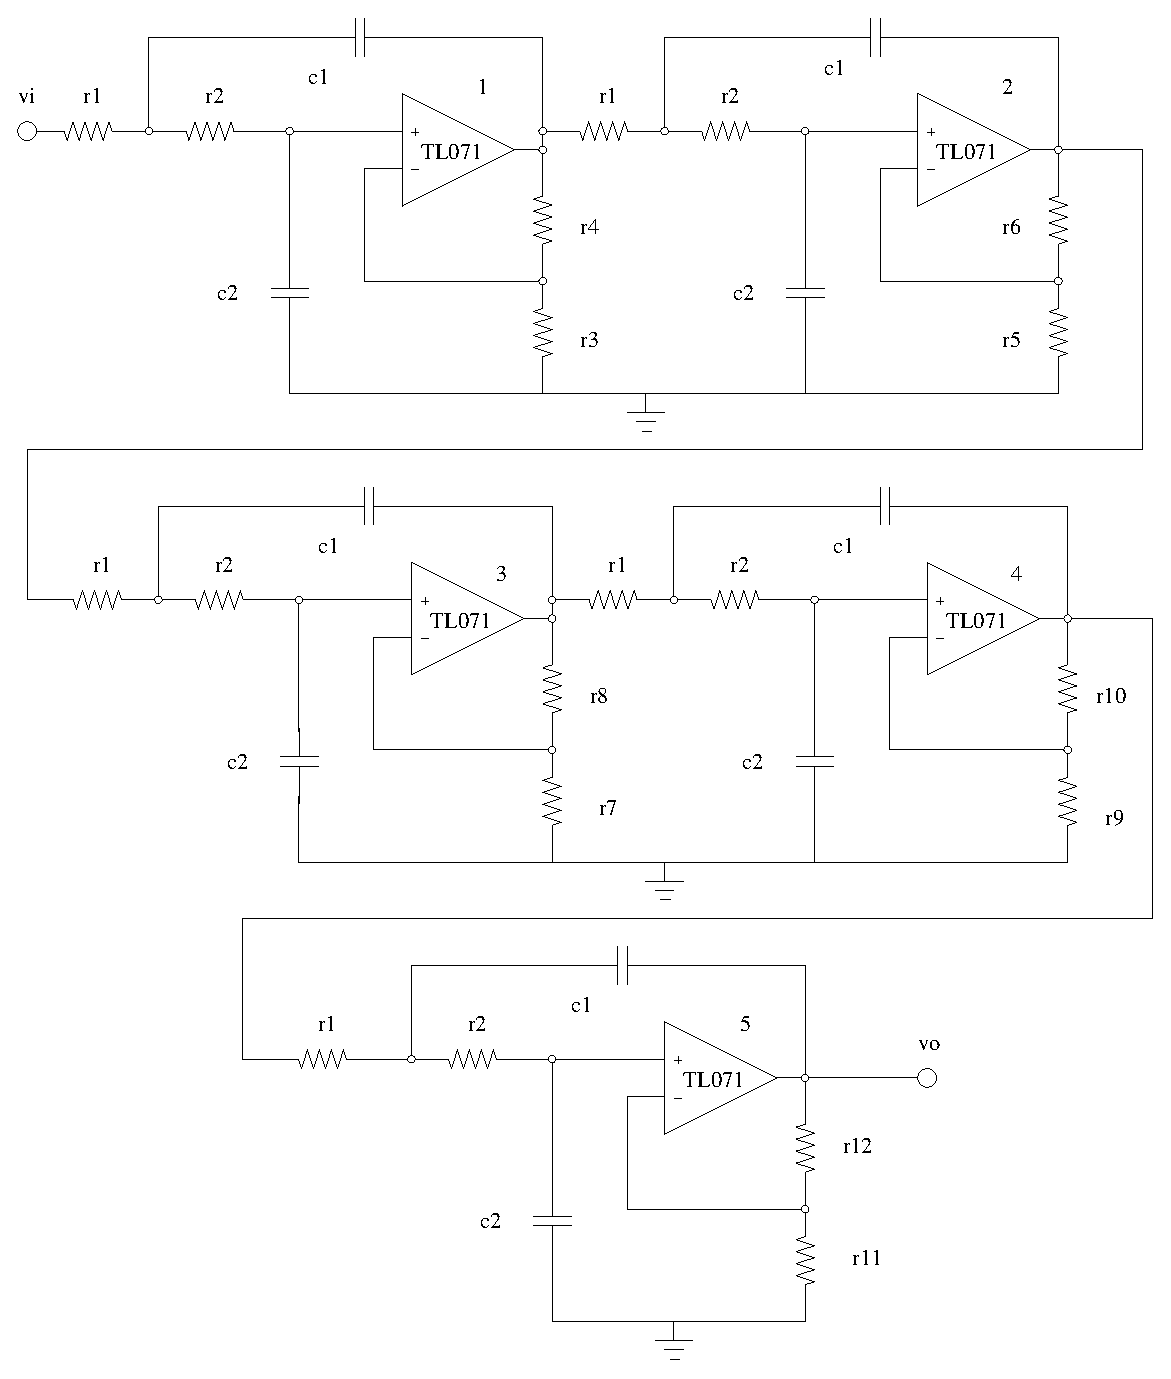
\includegraphics[width=\textwidth]{lp-imp.eps} 
	\caption{Ten-pole low-pass filter.}  
	\label{fig:lp-imp}
\end{figure}

Figure~\vref{fig:lp-imp} depicts the low-pass filter used in the
LLSPM. 

\begin{table}
\begin{center}	
	\begin{tabular}[htpb]{|c|c|l|l|} \hline
	Stage & Gain & Component & Value \\ \hline
	1& 1.586 & $C_1 = C_2$ & 2~$\mu$F \\
	 & 		 & $R_1 = R_2$ & 2.273~k$\Omega$ \\ 
	 &		 & $R_3$ & 10~k$\Omega$ \\
	 &       & $R_4$ & 5.8~k$\Omega$ \\
	2& 2.610 & $C_1 = C_2$ & 2~$\mu$F \\
	 & 		 & $R_1 = R_2$ & 2.273~k$\Omega$ \\ 
	 & 		 & $R_5$ & 10~k$\Omega$ \\
	 & 		 & $R_6$ & 16.1~k$\Omega$ \\
	3& 1.889 & $C_1 = C_2$ & 2~$\mu$F \\
	 & 		 & $R_1 = R_2$ & 2.273~k$\Omega$ \\ 
	 & 		 & $R_7$ & 10~k$\Omega$ \\
	 & 		 & $R_8$ & 8.9~k$\Omega$ \\
	4& 1.337 & $C_1 = C_2$ & 2~$\mu$F \\
	 &    	 & $R_1 = R_2$ & 2.273~k$\Omega$ \\ 
	 & 		 & $R_{9}$ & 10~k$\Omega$ \\
	 &  	 & $R_{10}$ & 3.4~k$\Omega$ \\
	5& 1.038 & $C_1 = C_2$ & 2~$\mu$F \\
	 &  	 & $R_1 = R_2$ & 2.273~k$\Omega$ \\ 
	 & 		 & $R_{11}$ & 100~k$\Omega$ \\
	 &   	 & $R_{12}$ & 3.8~k$\Omega$ \\
	\hline
	\end{tabular}
	\caption{Low-pass filter component values}
	\label{table:lp-filter}
\end{center}	
\end{table}

Table~\vref{table:lp-filter} summarizes the component values used in
the low-pass filter realization.


\subsection{LLSPM Amplifier design and implementation}
\label{secion:llspm-amp}
The total gain of the LLSPM must be in the order of $10^6$. A
amplification stage is applied to the signal at two different points
in the system. 

\begin{figure}[htbp]
\begin{center}
	\psfrag{+}[][]{+}
	\psfrag{-}[][]{-}  
	\psfrag{r1}[][]{$R_1$} 
	\psfrag{r2}[][]{$R_2$}
	\psfrag{r3}[][]{$R_3$}  
	\includegraphics*{amp1.eps}
	\caption{HP--filter output amplifier.}
\label{fig:hp-amp}
\end{center}
\end{figure}

\begin{table}
\begin{center}	
	\begin{tabular}[htpb]{|c|c|} \hline
	Component & Value \\ \hline
	$R_1$ & 10~k$\Omega$ \\
	$R_2$ & 200~k$\Omega$ \\
	$R_3$ & 200~k$\Omega$ \\
	\hline
	\end{tabular}
	\caption{High--pass filter amplifier component values}
	\label{table:hp-amp}
\end{center}	
\end{table}

The first amplifier, Figure~\ref{fig:hp-amp}, is applied to the output
of the high--pass filter output. It is necessary to lift the EEG
signal above the noise floor at the earliest possible stage. Even
though steps have been taken to reduce the DC signal component of the
AD620 output, a small DC offset value still exists. It is therefore
necessary to first remove the DC component with the high--pass filter
before amplifying the output signal in order to use the full supply
rail voltage range with a reduced risk of amplifier
saturation. Table~\ref{table:hp-amp} contains the component values of
Figure~\ref{fig:hp-amp}.


\begin{figure}[htbp]
\begin{center}
	\psfrag{+}[][]{+} 
	\psfrag{-}[][]{-} 
	\psfrag{r1}[][]{$R_1$} 
	\psfrag{r2}[][]{$R_2$}
	\psfrag{r3}[][]{$R_3$}  
	\psfrag{r4}[][]{$R_4$}  
	\psfrag{-vcc}[][]{$-v_{cc}$}  
	\psfrag{+vcc}[][]{$+v_{cc}$}  
	\includegraphics*{amp2.eps}
	\caption{LP--filter output amplifier.}
\label{fig:lp-amp}
\end{center}
\end{figure}

\begin{table}
\begin{center}	
	\begin{tabular}[htpb]{|c|c|} \hline
	Component & Value \\ \hline
	$R_1$ & 10~k$\Omega$ \\
	$R_2$ & 200~k$\Omega$ \\
	$R_3$ & 200~k$\Omega$ \\
	$R_4$ & 1~M$\Omega$ \\
	\hline
	\end{tabular}
	\caption{Low--pass filter amplifier component values}
	\label{table:lp-amp}
\end{center}	
\end{table}

The second amplifier, Figure~\ref{fig:lp-amp} amplifies the signal at
the low--pass filter output. The five operational amplifier stages
introduces a small DC offset on top of the output signal which is
removed by the voltage divider $R_4$. Table~\ref{table:lp-amp}
contains the component values of Figure~\ref{fig:lp-amp}.

\subsection{LLSPM Integration}
\begin{figure}[htbp]
\begin{center}
	\psfrag{ia}[][]{IA}  
	\psfrag{ae1}[][]{$ae_{1}$}  
	\psfrag{ae2}[][]{$ae_{2}$}  
	\psfrag{lp}[][]{LP}  
	\psfrag{hp}[][]{HP}
	\psfrag{lpa}[][]{LPA}
	\psfrag{hpa}[][]{HPA}
	\psfrag{o}[][]{O}       
	\psfrag{rld}[][]{RLD}  
	\psfrag{dc}[][]{DC}  
	\psfrag{g}[][]{g}  
	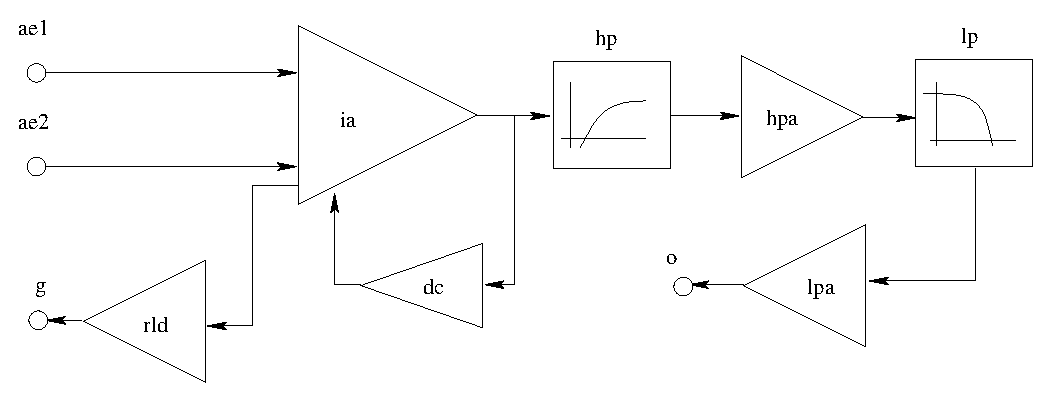
\includegraphics[width=\textwidth]{llspm-int.eps}
	\caption{LLSPM Integration.}
\label{fig:llspm-int}
\end{center}
\end{figure}

Figure~\ref{fig:llspm-int} is a signal flowchart of the complete low
level signal processing module. The instrumentation amplifier's (IA)
inputs are fed via two active electrodes ($ae_{1}$, $ae-{2}$). A mean
value of the input difference are amplified and fed back to the skin
surface via the right-leg drive (RLD) circuit. The IA output is
sampled, integrated and fed to the IA's reference pin via the DC
circuit. This reduces the DC value of the output signal. The IA output
is filtered through a HP filter (HP) to reduce the signal DC component
further before amplified by the high--pass filter amplifier (HPA). The
HPA output signal is passed through a low--pass filter (LP) before
being amplified by the low-pass amplifier (LPA).

The output signal (O) is a amplified and filtered version of the
difference signal between $ae_{1}$ and $ae_{2}$.


\subsection{LLSPM Container implementation}
\begin{figure}[htbp]
\begin{center}
	\includegraphics*{whole-system1.ps}
	\caption{LLSPM Container.}
\label{fig:llsp-container}
\end{center}
\end{figure}

Figure~\ref{fig:llsp-container} depicts the LLSPM container used in
the project. The LLSPM container was made using a commercially
available 'mini--tool-box'. The box is made out of 0.5~mm plate metal
which makes the mounting of sockets relatively easy. The box also
functions as a Faraday cage shielding the circuit boards against
EMI. The signal sources of the SME were also housed in the LLSPM
container. This arrangement made the injection of test signals into
the LLSPM circuits relatively easy. The necessary access holes were
drilled and the signal and power connections mounted on the container
exterior. Care was taken to ground all external wiring and shielding
to the container's metal walls.



\section{LLSP noise analysis}
The filters employed in the LLSP module contributes noise and signal
error components to the resulting filtered EEG signal. The error
signal components are once more divided in two categories:
\begin{itemize}
	\item Intrinsic noise generated within the filter modules.
	\item External interference or signal errors not associated with
	random charge movement in the filter circuit components.
\end{itemize} 


\subsection{Intrinsic noise errors}
Inaccuracies of the theoretical approximation of filter action is the
most significant cause of unexpected erroneous system response
\cite[p18]{design-guide}.

For microvolt-level signal acquisition systems broad-band noise
contribution by active filter components pose a significant threat to
the system SNR \cite[p38]{mvl-data}. Later filter stages remove stop
band noise components from earlier stages but does not affect
pass-band noise. The netto effect is a steady increase in pass-band
noise contributed by each filter stage. It is necessary to
significantly amplify the EEG signal at an early stage reducing the
influence of added system noise in proceeding filter stages. Noise
levels peak at filter corner frequencies depending on the filter's
quality factor $Q$.

Non-linear action in the filter circuit response mixes EEG frequency
components up and down leading to harmonic distortion in the filter
output signal. Distortion levels varies with the frequency and
amplitude of input signals. Second and higher order harmonics are
filtered out for frequencies near the filter's corner frequency. The
loop gain of the operational amplifier used in the filter realization
is sufficient to reduce distortion to acceptable levels
\cite[20]{design-guide}.


\subsection{External interference}
The various filter stages are also possible injection points of
external interference. External noise signals are coupled into the
filter circuit as discussed previously in
Section~\vref{section:passive-analyses} and illustrated in
Figure~\vref{fig:electrode-noise}. The amount of external interference
entering the system via the filtering stages are minimized by applying
standard shielding and decoupling techniques.

Cabling is susceptible to induced noise interference and is shielded
as far as possible. Woven--braid twisted--pair shielding is used as it
provides a superior EMI shield \cite[39]{mvl-data}.

The LLSPM is contained in a single shielded metal container and
physically attached to the signal acquisition module container. The
connecting signal cables are kept as short as possible, not exceeding
1~m. Above measures serves to keep external interference to a minimum.


